\section*{Practical 4: The Angular Distribution in Python }

For this practical, your task will be to implement the remaining code to reproduce some results for the $e^+e^-\to q\bar{q}g$. Particularly, we would like to reproduce the real emission plot - the distribution of events with respect to angle. Recall that at leading order, with no gluon emission, we expect the relative angle between quarks to be $\pi$: they should scatter in opposite directions. As we introduce gluons if we allow gluons in our final state, the angle will be slightly reduced as the gluon will carry some of the momentum. As the gluon becomes soft, the angle will restore to $\pi$. We would like to see the exact distribution of angles after implementing a soft cut. 
Create a new file for our experiment, \codeinline{rratio_differential.py}. We rename the function to \codeinline{rratio_differential}. In \codeinline{run.py}, add this experiment to the cases, as well as the appropriate code to the parser. We will also need to import the file so that \codeinline{run.py} knows where to find our code,
\begin{codeenv}
    from CHEP.experiments.rratio_differential import rratio_differenital
\end{codeenv}
We would like to plot a histogram. How do we gather the data we need for plotting? If we look inside our integrand function, we can see the where we generate our data and add to our evaluations. This is where we can start gathering angular data. The simplest way is to add a new argument to our integrand function, which allows it to take an array as input. Note that one should take care when doing this: when we pass an object into a method, depending on the coding language, it can either be a reference to the object's location in memory or copy? If it were a copy, the object will only be modified in the scope of the method, and our original object will be unmodified. This isn't good if we're trying to store data. We want reference for the histogram. This is the default in python - exactly what we want. However, if we want to parallelise, this would make things more difficult as the code would try and modify our array concurrently - though we won't worry about this for now. Let's create an array for our data:
\begin{codeenv}
       costheta_histo=[0.0 for _ in range(200)]
\end{codeenv}
This gives 200 bins. We could also add an option for number of  bins in our experiment run parameters, but for now we will keep things simple. We then edit our integrand constructor to take this vector as an item by adding a parameter \codeinline{histo}. Inside the integrand method, we can assign our generated phase space point to a set of variables to save the momenta 
\begin{codeenv}
    p_ep, p_em,p_d,p_db,p_g=ps_point
\end{codeenv}
We can then compute the angle between our quarks
\begin{codeenv}
    costhetaqq=p_d.space().dot(p_db.space())/(abs(p_d.space())*abs(p_db.space()))
\end{codeenv}
We would then like to assign this to a bin. To do so, we should round the angle down to an appropriate number based on the number of bins. Noting that \codeinline{int} casting in python is the same as taking the \codeinline{floor}, then
\begin{codeenv}
    bin_id=int((1+costhetaqq)/2*len(histo))
\end{codeenv}
Note that we also need to account for the weight, since we don't have unweighted events. We can save these weights with
\begin{codeenv}
            histo[bin_id][0]+=wgt
\end{codeenv}

A differential distribution is defined for a given observable function $J(\phi)$ of the final-state kinematic configuration $\phi$, which in case reads:
\begin{equation}    
J(\phi) \equiv \cos\theta_{q\bar{q}}(\phi) := \frac{\vec{p}_q\cdot \vec{p}_{\bar{q}}}{|\vec{p}_q||\vec{p}_{\bar{q}}|}
\end{equation}
The formal definition of the differential cross-section for this observable function $J(\phi)$ is:
\begin{equation}    
\frac{d \sigma}{d J} := \int d \phi |\mathcal{M}(\phi)|^2 \delta \left( J(\phi) - J \right)
\end{equation}
In order to solve this integral analytically, one would have to be able to express the observable $J$ in terms of the phase-space parameterization variables supporting $\phi$, which is not always possible, especially for complicated observables. Not to mention that one may be interested in monitoring a vast ensemble of different observable at the same time for a given simulation.
It is therefore convenient to instead consider a piece-wise constant approximation of the truly continuous differential distribution $\frac{d \sigma}{d J}$, by constructing histograms instead, with a certain number of bins, each identified with a boundary $b_{i,\text{min}}$ and $b_{i,\text{max}}$. The value of the piece-wise constant function within such an interval, i.e. the "height" $h_i$ of this bin of the histogram, is then:

\begin{equation}
\label{histo}
h_i := \int_{b_{i,\text{min}}}^{b_{i,\text{max}}} dJ \left( \frac{d \sigma}{d J}\right) = \int d \phi |\mathcal{M}(\phi)|^2 \Theta \left[ J(\phi) -b_{i,\text{min}} \right] \Theta \left[b_{i,\text{max}}-J(\phi) \right]
\end{equation}
Notice that it is clear that if the total range of the histogram covers the complete final-state phase-space, then the following propery holds:
\begin{equation}    
\sum_i h_i = \sigma_{\text{tot}}
\end{equation}

This expression~\eqref{histo} is well-suited to be evaluated numerically independently of any choice for the phase space-parameterization. It can essentially be understood as the estimator for the cross-section within a fiducial volume identified by the bin of interest, and during the Monte-Carlo integration, one can simply test whether or not a given sample point belongs to the interior of the bin range.

However, as for any estimator of the central value of an integral, one must normalize the sum of all sample weights by the number of sample points entering that bin, which we must therefore keep track of as follows:
\begin{codeenv}
        costheta_histo=[(0.0, 0) for _ in range(200)]
\end{codeenv}
and change 
            \begin{codeenv}
histo[bin_id][0]+=wgt
histo[bin_id][1]+=1
            \end{codeenv}
\color{black}
We can use this information to appropriately normalise each bin
\begin{codeenv}
        normalise_histo=[(tot_wgt/n_events) if n_events>0 
        else 0 for (tot_wgt,n_events) in costheta_histo ]
\end{codeenv}
which we can then plot
\begin{codeenv}
    bins=np.linspace(-1,1,len(normalise_histo))
    plt.bar(bins,normalise_histo, width=0.01)
    plt.show()
\end{codeenv}
As mentioned at the beginning, the resulting distribution will depend on our gluon cut. By setting this to a relatively high energy to remove the soft gluons, for example \codeinline{GLUON_ENERGY_CUT = 300.0} we can obtain a plot for the angular distribution.
\begin{figure}[H]
    \centering
    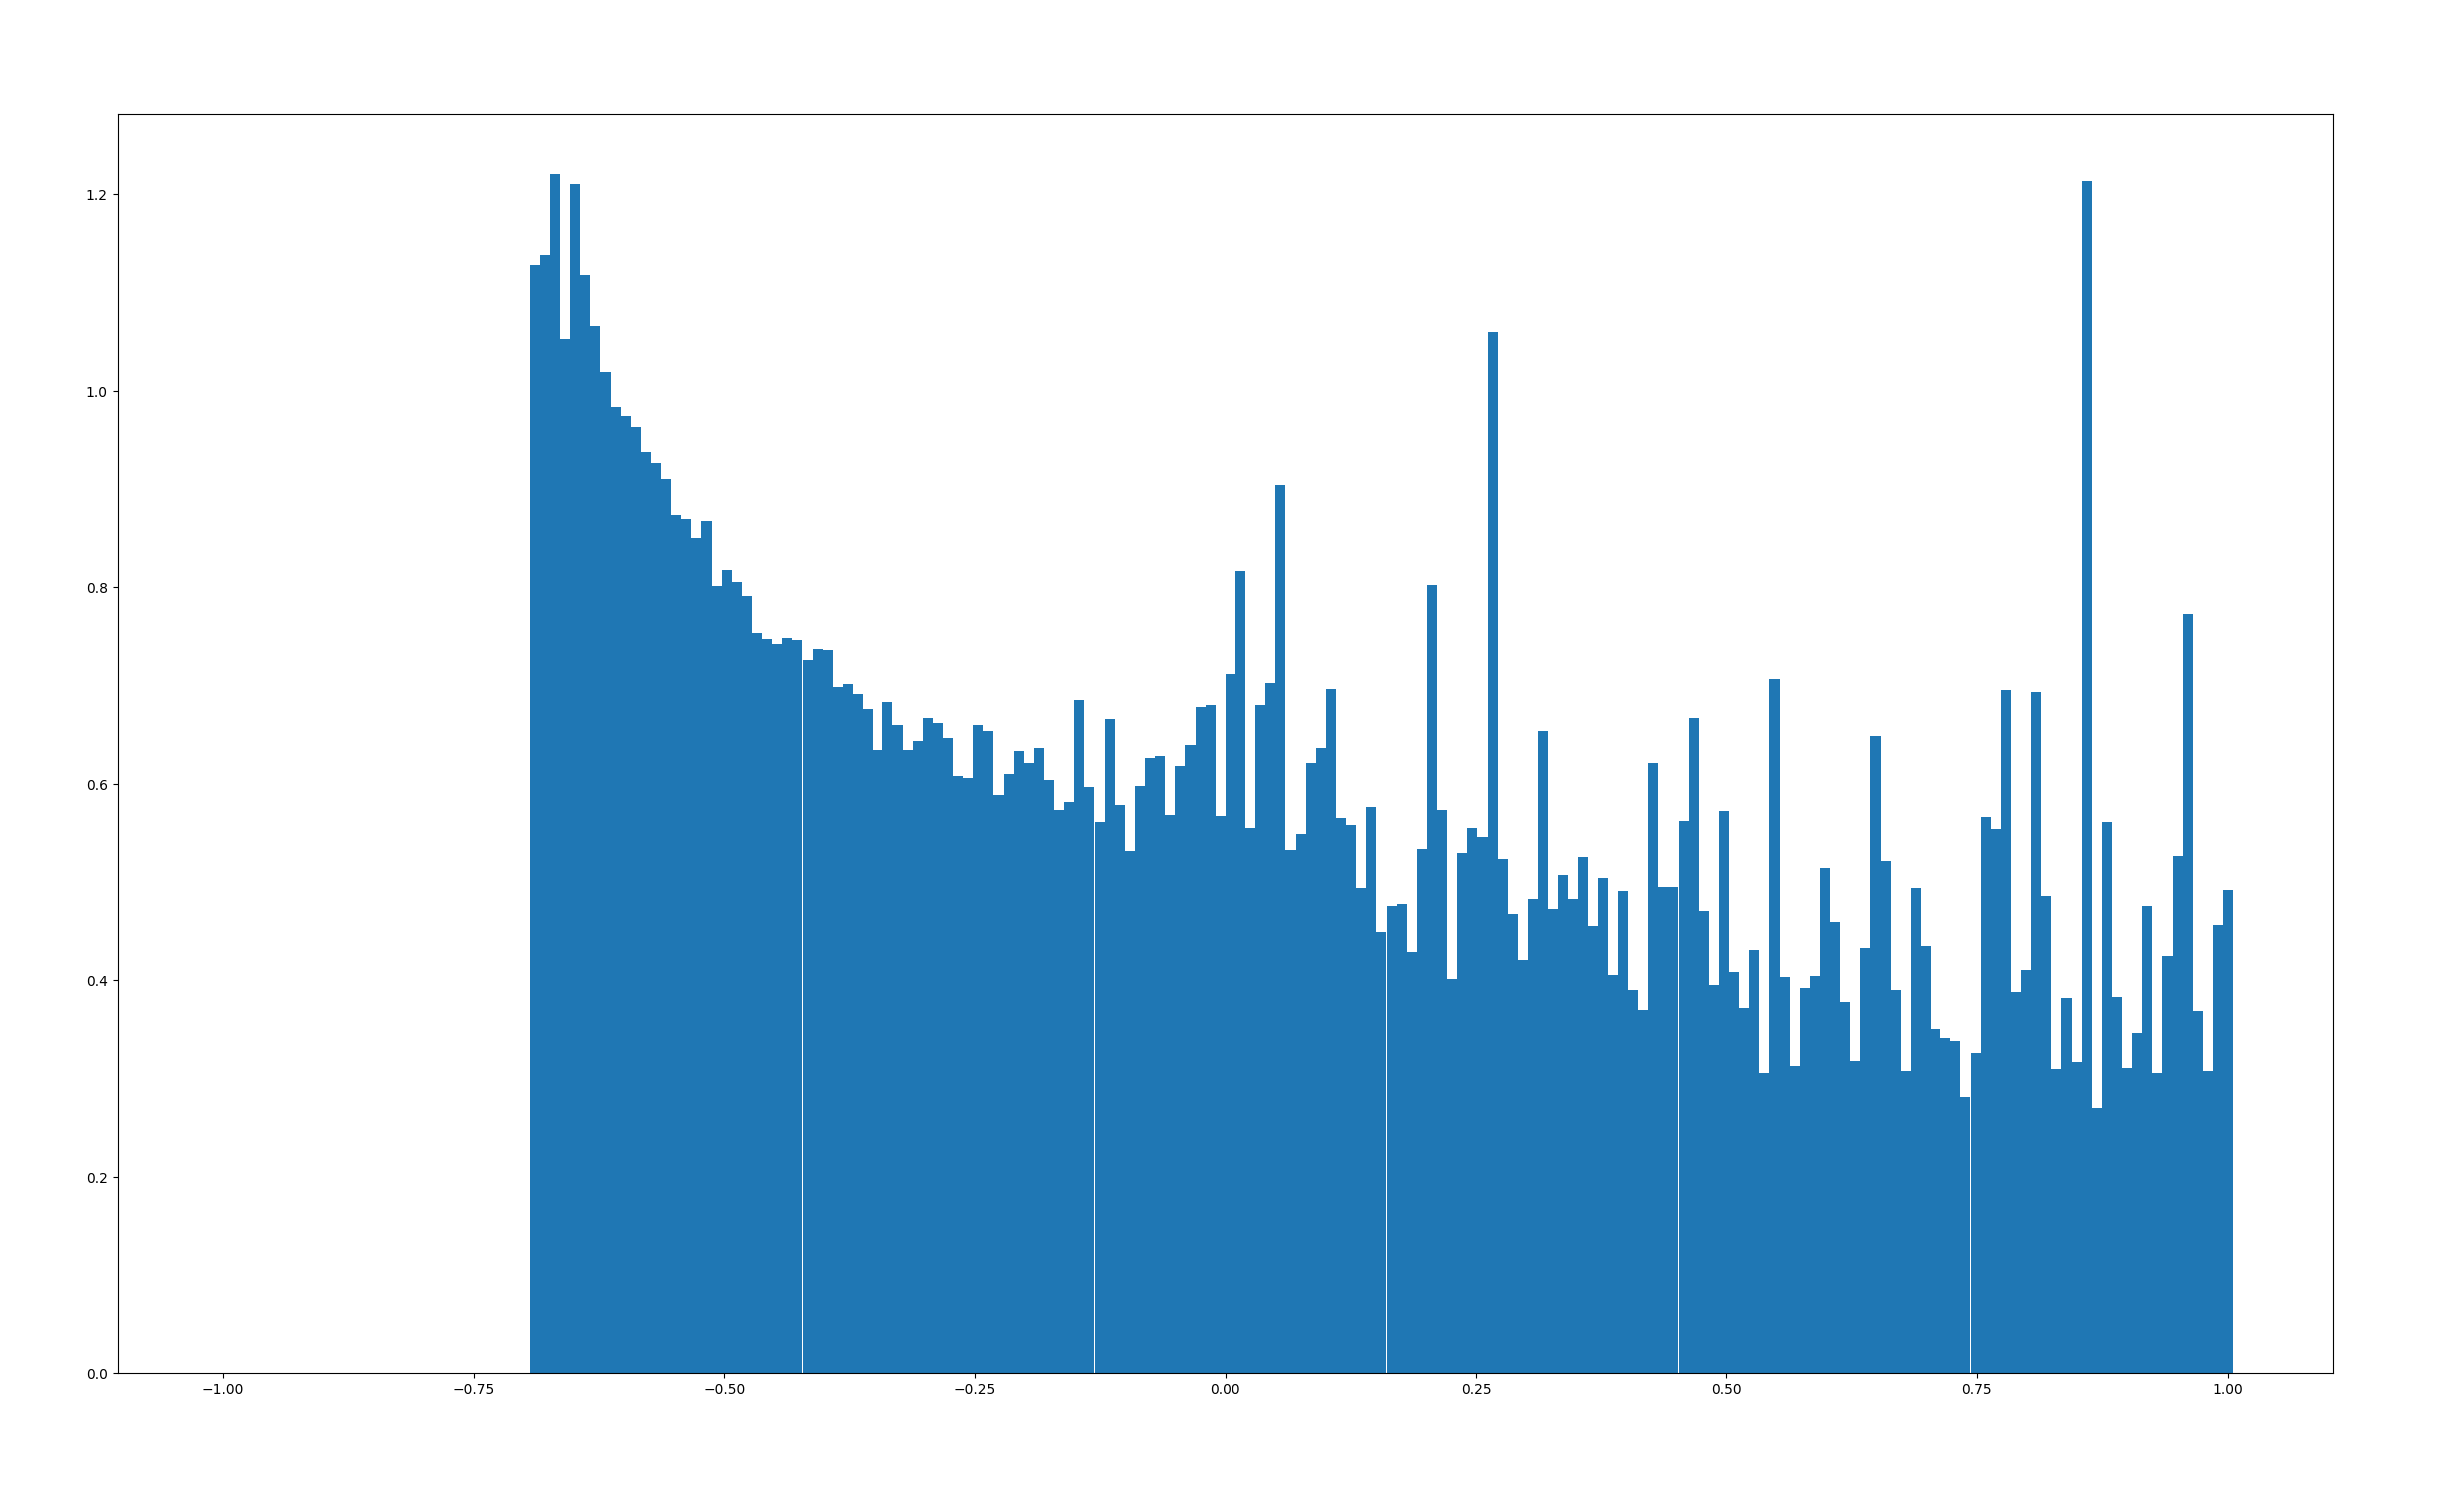
\includegraphics[width=0.75\linewidth]{tex/ims/angular_dist.png}
    \caption{Cross-section angular distribution for the 300 GeV soft gluon cut.}
    \label{fig:enter-label}
\end{figure}
Observe that the distribution close to $\cos(\theta)=-1$ is quite well resolved, while at $\cos(\theta)=1$ the histogram is much more jagged and noisy. This is an artefact of our sampling: we generate far more points closer to $\theta=\pi$ and thus have better resolution.
